%\begin{frame}{ASPDAC feedback}
%\begin{itemize}
%\item Need not work on routing, because generally routing overhead will grow proportionally to gate-level area overhead
%\item Till now, only quantified increase in number of gates in the SAT instance, did not actually run the SAT solver and verify the results
%\end{itemize}
%\end{frame}

\begin{frame}{Sequential Locking and SAT-solving}
	\begin{table}[!htbp]
		\begin{center}
			\caption{SAT-attack on Scan-unrolled Sequentially Locked c880 circuit}
			\label{tab:sat-attack}
			\begin{tabular}{|c|c|}
				\hline
				\# Scan cells (added at primary outputs) encrypted & Decryption time \\
				\hline
				0 & 3.49s \\
				\hline
				11 & 9.46s \\
				\hline
				16 & 45.86s \\
				\hline
				20 & 100.88s \\
				\hline
				24 & 250.48s \\
				\hline
			\end{tabular}
		\end{center}
	\end{table}
	\begin{itemize}
%		\item The correct key decryption was SUCCESSFUL when SAT-attack launched on combinational circuit
		\item Also, the correct key decryption was \alert{UNSUCCESSFUL} 
			\begin{enumerate}
			\item Actual combinational key=000000110011111011110110110101011001000100000011110000011010000111111111100101101101100110111001010000010011110010111111011001010000011110110011101011111010010100010101110000010110011111110100
			\item Decrypted combinational key=000000110011111011010110110101000001001000000011100011111010000100101111100100001101001010111000110000010011110110111111011001010000001110110011101011111010010100010101010000010010001110000000
			\end{enumerate}
	\end{itemize}
\end{frame}

\begin{frame}{Explanation using small example}
\begin{figure}
	\begin{center}
		\caption{Original s27 circuit}
		\label{fig:s27}
		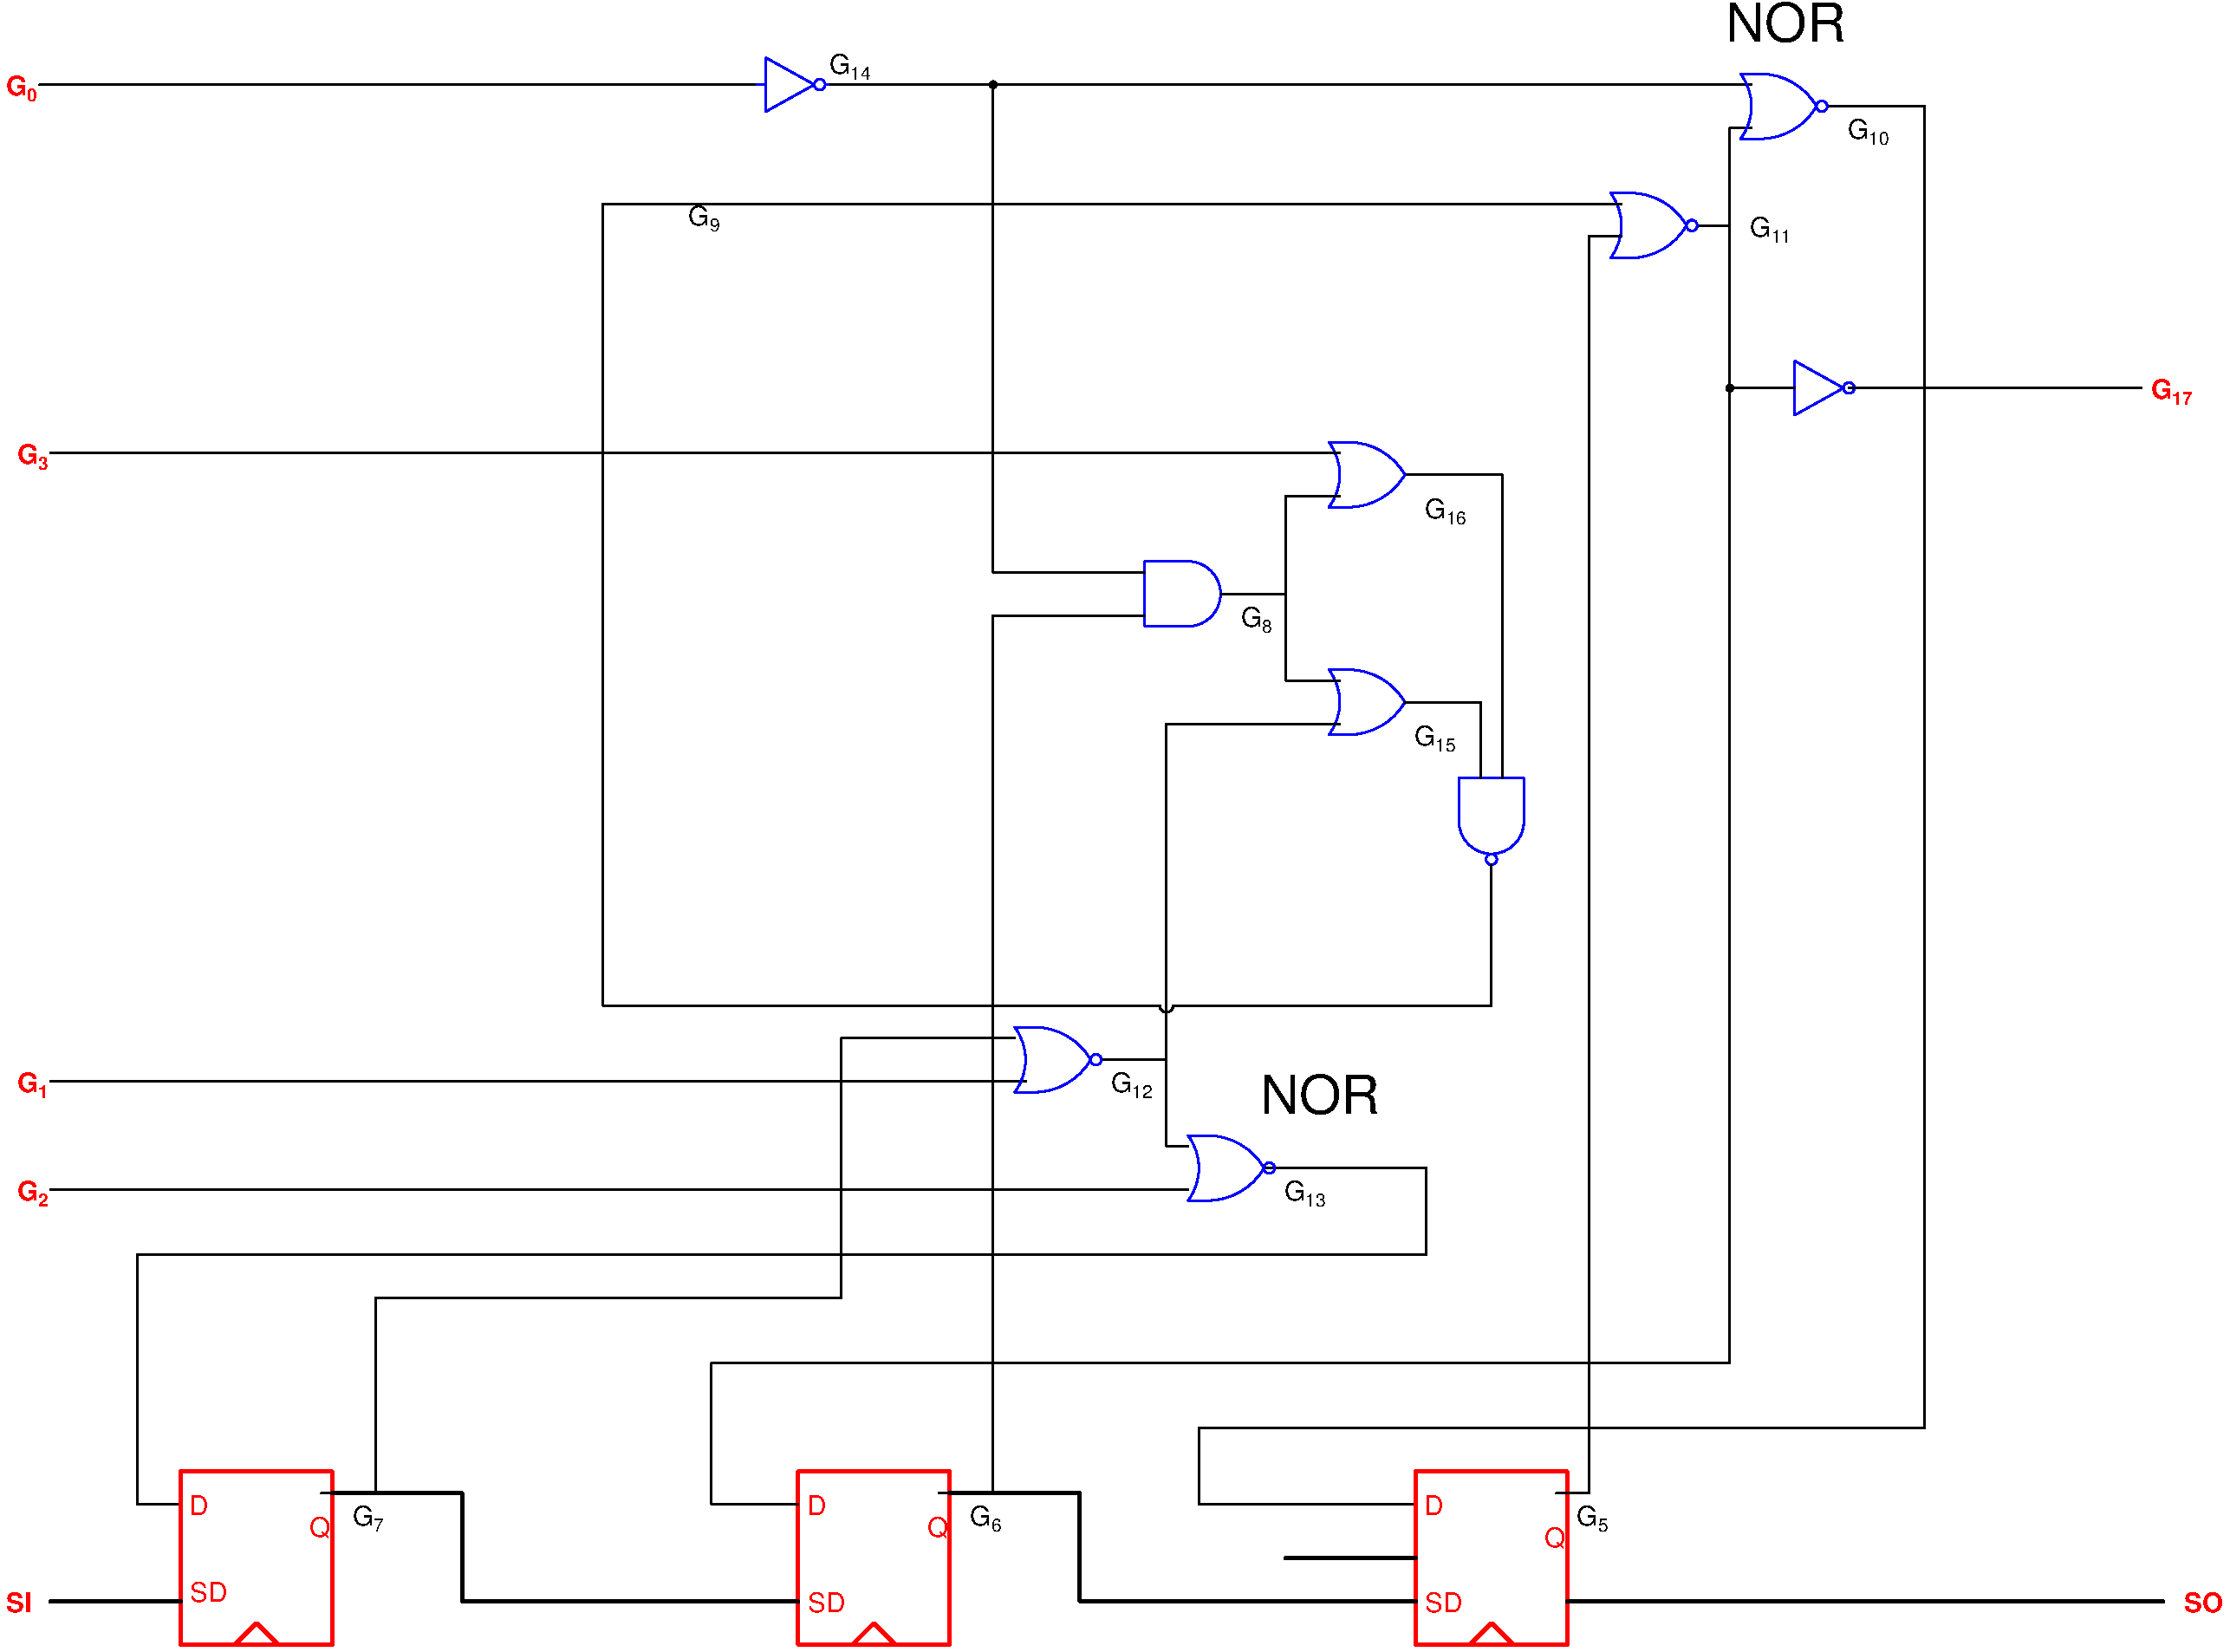
\includegraphics[scale=0.15]{fig/s27_original.pdf}
	\end{center}
\end{figure}
\end{frame}

\begin{frame}{Explanation using small example}
\begin{figure}
	\begin{center}
		\caption{Sequentially Locked s27 circuit}
		\label{fig:s27-locked}
		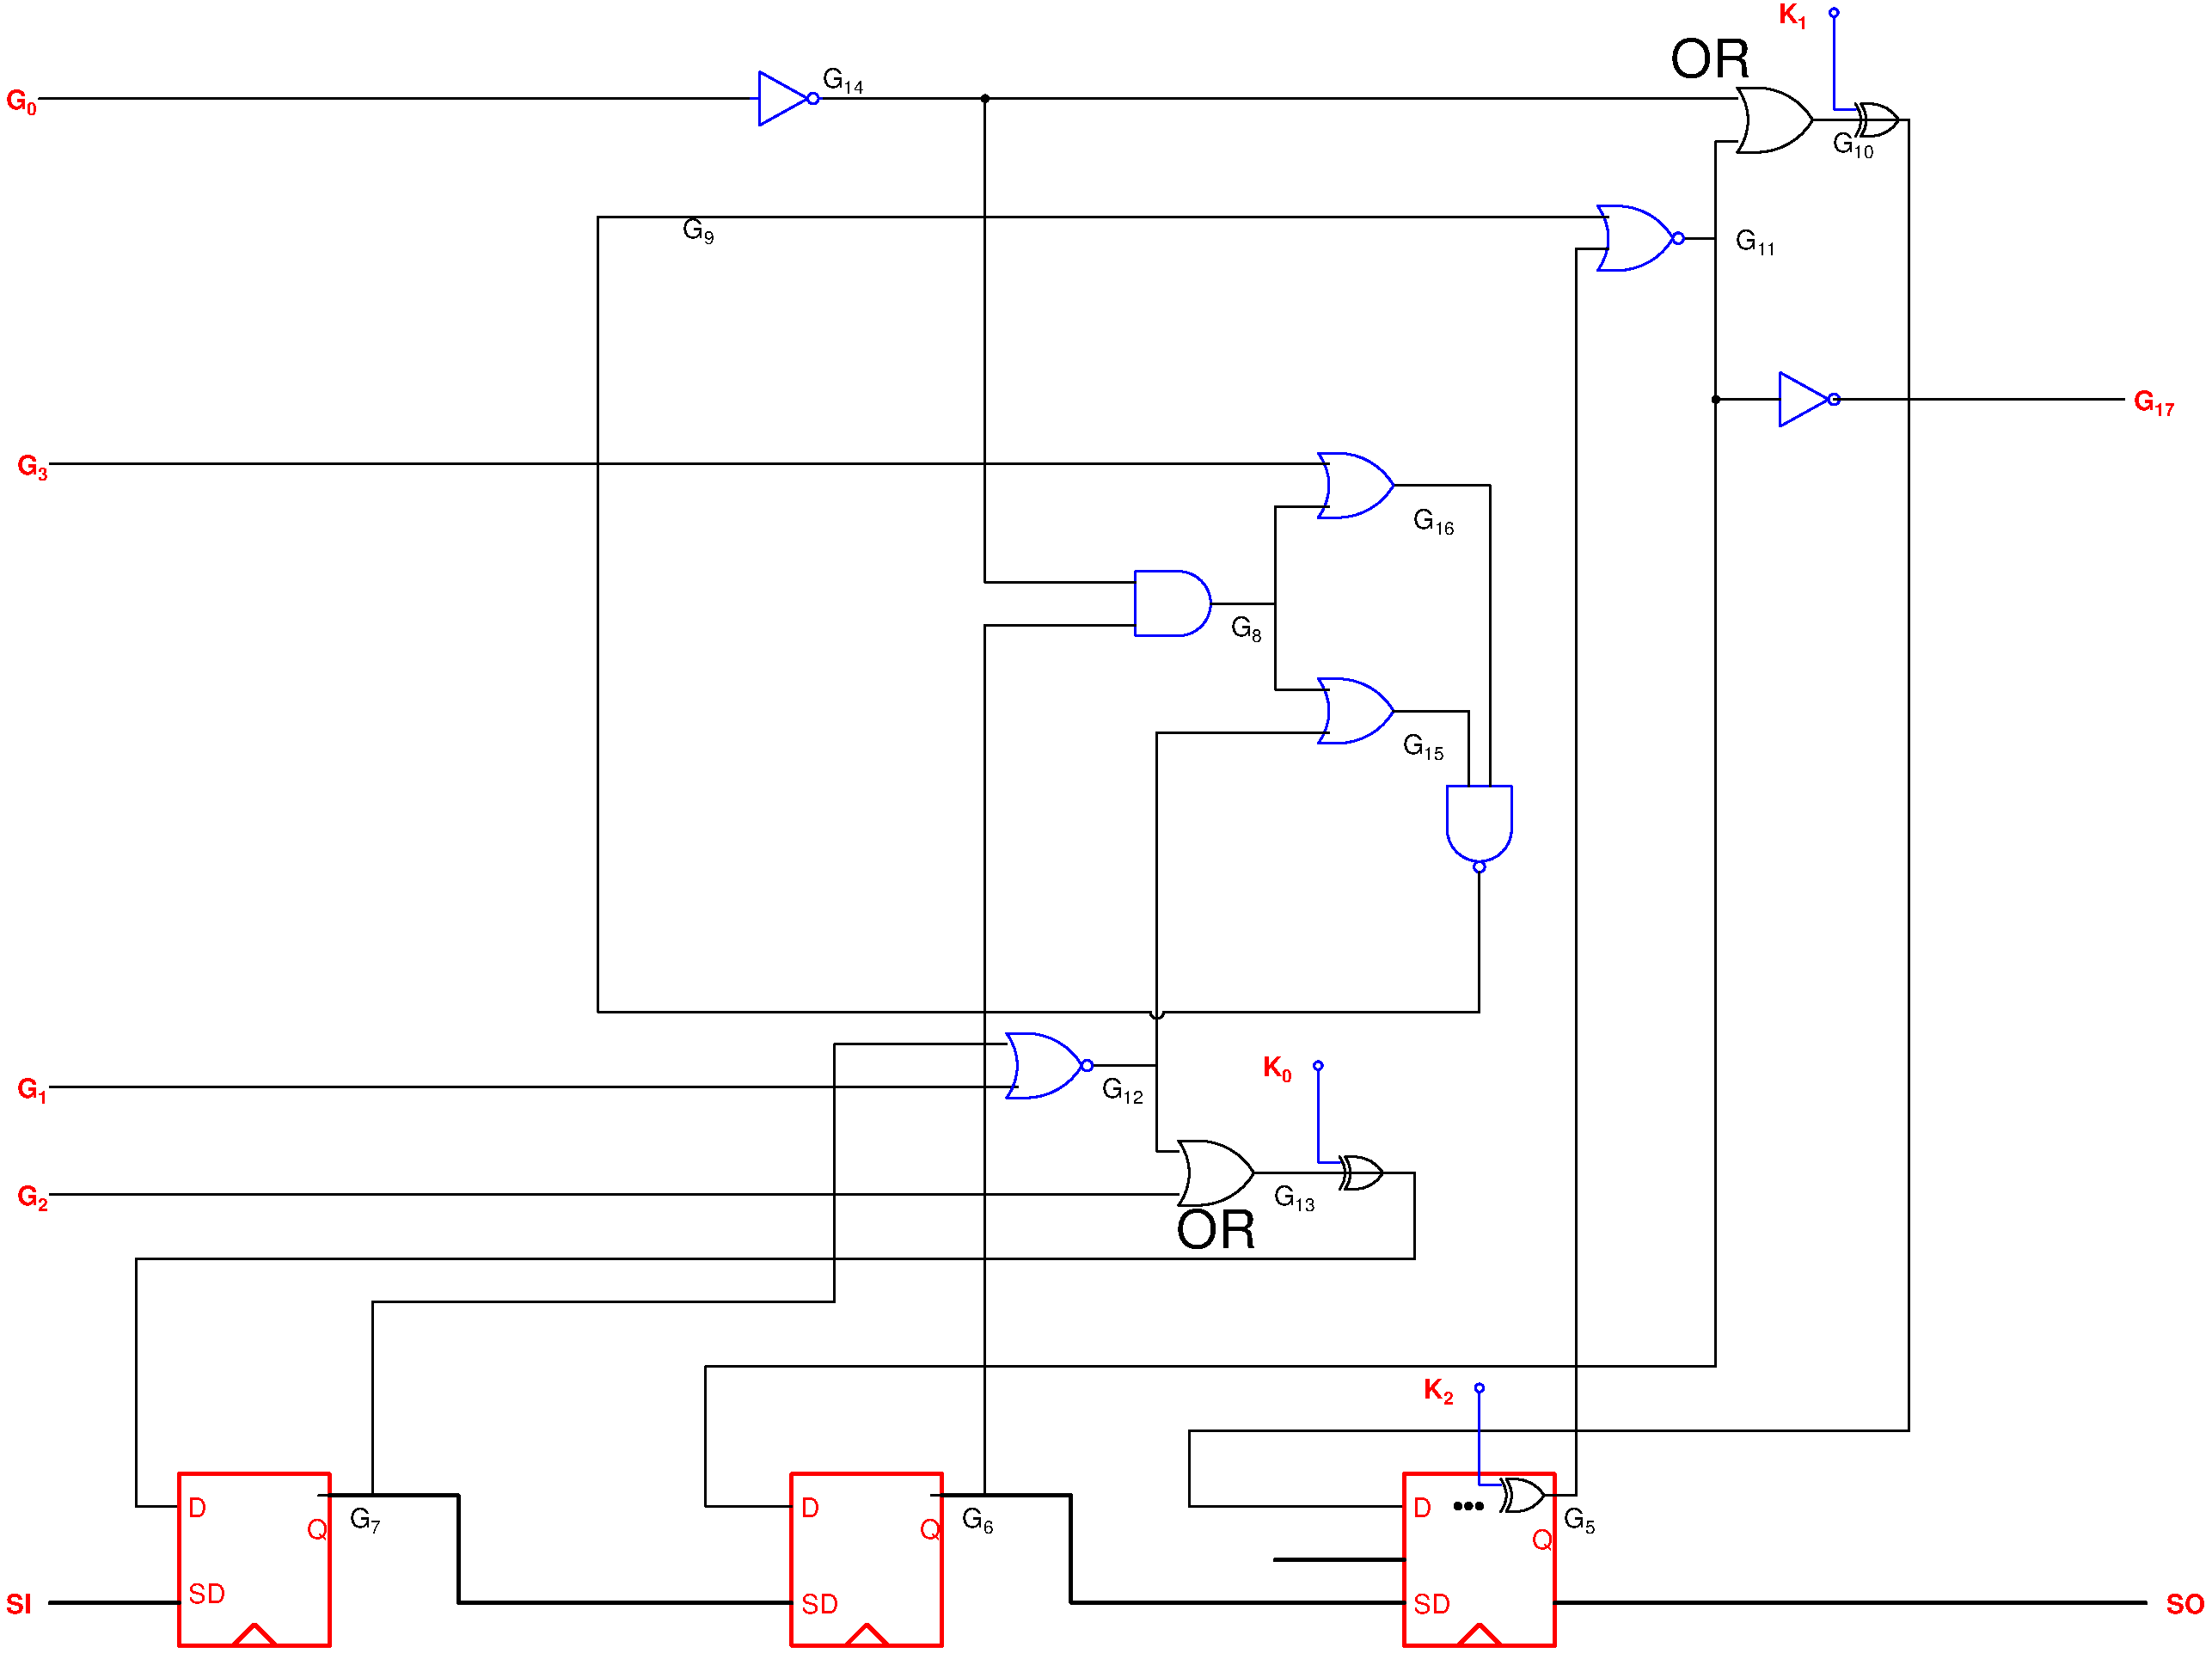
\includegraphics[scale=0.15]{fig/s27_locked.pdf}
	\end{center}
\end{figure}
\end{frame}

\begin{frame}{Explanation using small example: Equivalence classes of Keys}
\begin{itemize}
\item $\{K_0, K_1, K_2\}=110$ is a valid key
\item $\{K_0, K_1, K_2\}=001$ is also a valid key
\item Thus, scan-chain locking helped produce equivalence classes of keys, that cannot be distinguished
\item So, the attacker is unable to decrypt the correct key using SAT-attack
\item Hence, sequential locking is able to achieve SAT-attack Resilience in two ways:
	\begin{enumerate}
		\item Decryption of wrong keys during SAT-attack
		\item Increase in SAT-attack runtime by 1-2 orders of magnitude
	\end{enumerate}
\end{itemize}
\end{frame}
